\chapter{Operating Systems}

\section{Introduction}
The operating system in a computer acts as the intermediary between the hardware and the applications that allow the user to utilize that hardware for meaningful purposes such as playing games, browsing the internet, graphic design, and many other activities.

The operating system is similar to the control unit in a car. A car has an engine, fuel tank, wheels, brakes, and so on. But without the control unit, the car would be nothing more than a collection of mechanical parts connected together.

\begin{minipage}[c]{0.6\textwidth}
	\subsection{Computer System Components}
	A computer system does consist of 4 main layers to operate, take out one of them and what is left can not be a computer system
	\begin{itemize}
		\item \textbf{Hardware}\\
		computing and storing resources such as (CPU, GPU, memory units, I/O devices)
		\item Operating System\\
		manage the computer's resources (Hardware) and makes a mid
		\item Application
		define the ways in which the system resources are used to solve the computing problems of the users (compilers, database systems, video games, business programs)
		\item User
		\begin{enumerate}
			\item human
			\item machine
			\item other computers
		\end{enumerate}
	\end{itemize}
\end{minipage}%
\hfill
\begin{minipage}[r]{0.40\textwidth}
	
	\begin{figure}[H]
		\centering
		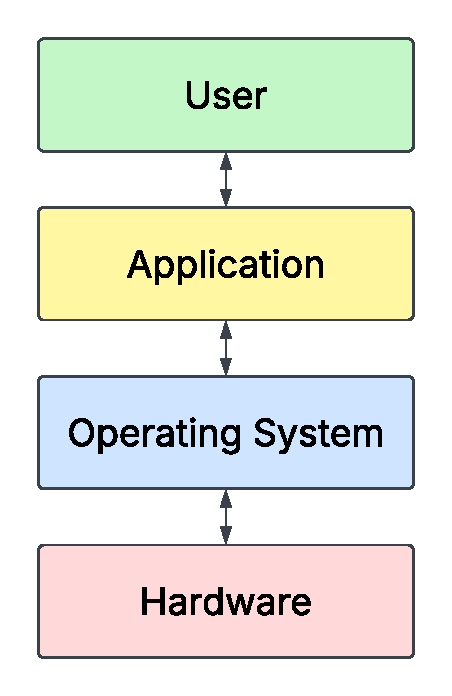
\includegraphics[width=0.8\linewidth]{figures/OS block 1}
		\caption{Computer layered architecture diagram}
		\label{OS1}
	\end{figure}
\end{minipage}


\section{Von Neumann Architecture}
Von Neumann architecture Figure[\ref{fig:von}] was first published by John von Neumann in 1945

His computer architecture design consists of a Control Unit (CU), Arithmetic and Logic Unit (ALU), Memory Unit, Registers and Inputs/Outputs.



\begin{minipage}[c]{0.6\textwidth}
	\subsection{Central Processing Unit (CPU)}
	The Central Processing Unit (CPU) is the electronic circuit responsible for executing the instructions of a computer program. It is sometimes referred to as the microprocessor or processor.
	The CPU contains the ALU, CU and a variety of registers.
	\\
	\subsubsection{Registers}
	Registers Figure[\ref{fig:reg}] are high speed storage areas in the CPU. All data must be stored in a register before it can be processed.\\
		
	\begin{tabular}{p{1.5cm}p{3cm}p{3.5cm}}
		\toprule
		Abb & Meaning & Function \\
		\midrule
		MAR & Memory Address Register & Holds the memory location of data that needs to be accessed \\&&\\
		
		MDR&Memory Data Register&Holds data that is being transferred to or from memory\\&&\\
		
		AC&Accumulator&Where intermediate arithmetic and logic results are stored\\
		PC&Program Counter&Contains the address of the next instruction to be executed\\&&\\
		
		CIR&Current Instruction Register&Contains the current instruction during processing\\ \bottomrule & \captionof{table}{Registers}&\\
		
		
	\end{tabular}
\end{minipage}
\hfill
\begin{minipage}[r]{0.40\textwidth}
	
	\begin{figure}[H]
		\centering
		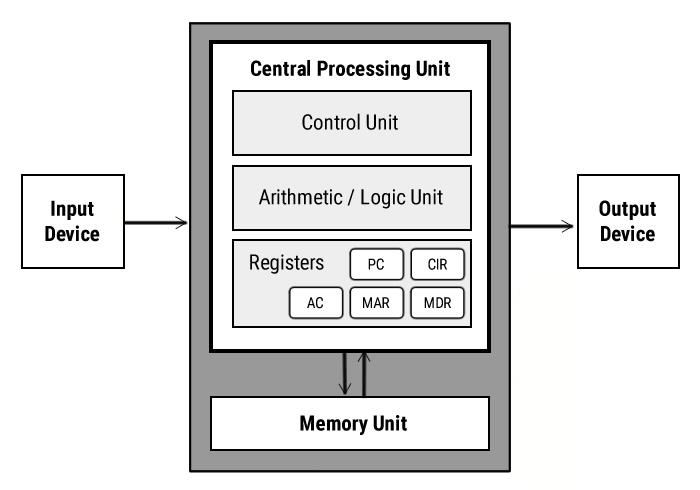
\includegraphics[width=1\linewidth]{figures/Von}
		\caption{Von Neumann Architecture}
		\label{fig:von}
	\end{figure}
	\begin{figure}[H]
		\centering
		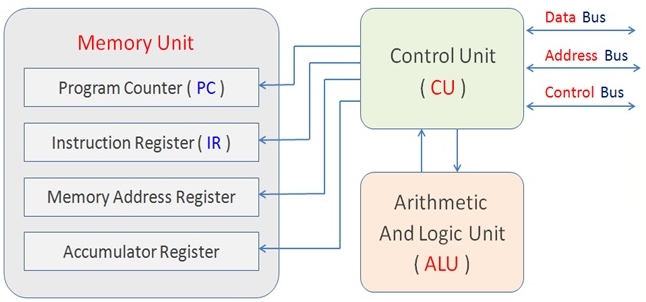
\includegraphics[width=1\linewidth]{figures/reg}
		\caption{}
		\label{fig:reg}
	\end{figure}
	
\end{minipage}

\subsubsection{Arithmetic and Logic Unit (ALU)}


